\section{Umsetzung}

\subsection{Überblick}


In dieser Masterarbeit wird unsere Applikation über die RPC Schnittstelle eines Full Nodes an das Ethereum-Netzwerk angebunden. Dies ist in Abbildung \ref{fig:ethereum_integration} verdeutlicht.
 
\begin{figure}
\centering
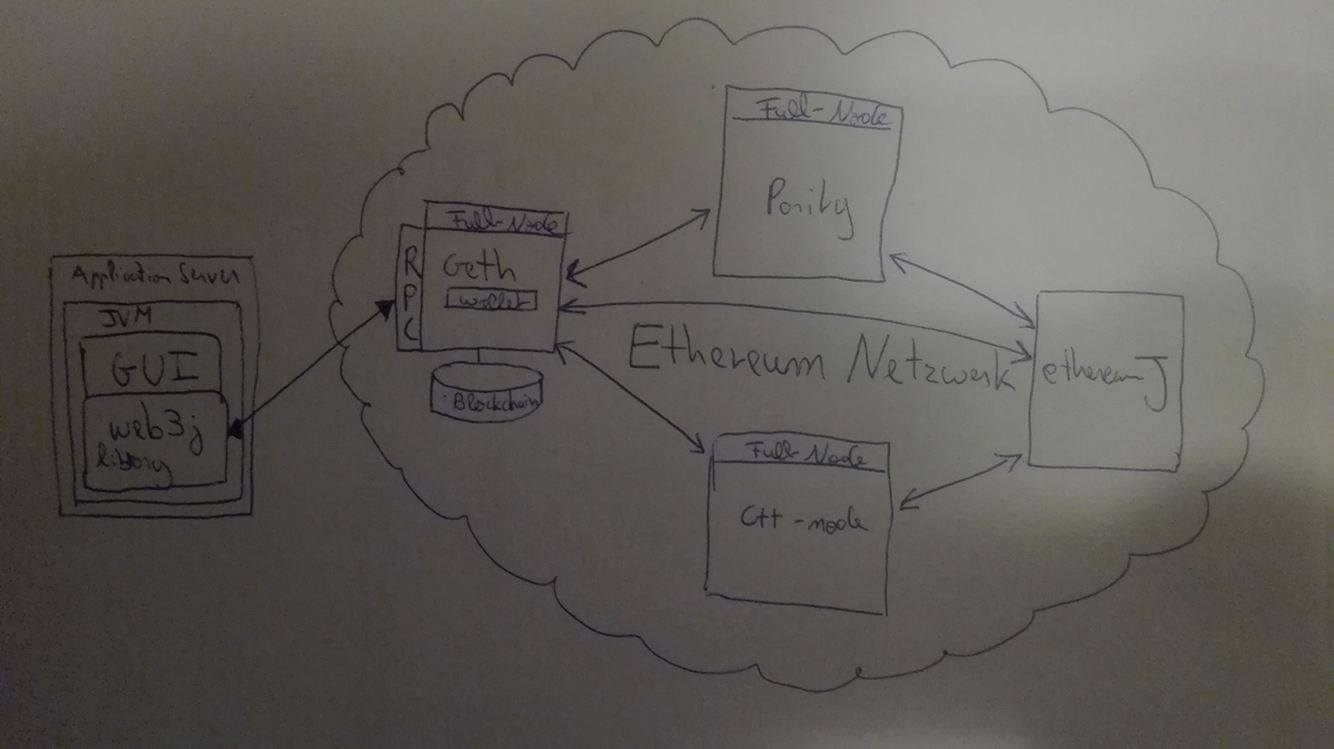
\includegraphics[width=1\linewidth]{Figures/ethereum_integration}
\decoRule
\caption{Ethereum: Netzwerk Integration}
\label{fig:ethereum_integration}
\end{figure}


\subsection{Smart Contract}
Die folgenden Codestücke beschreiben den TrustlessGambling Smart Contracts in der Sprache Solidity.
\subsubsection{Datenmodell}

\begin{lstlisting}[basicstyle=\small]
pragma solidity ^0.4.0;
contract TrustlessGambling {
    // constants
    uint8 public constant NBR_OF_SLOTS =3;
    uint public constant EXPECTED_POT_AMOUNT=1000;// WEI
    uint8 public constant PAYOUT_BLOCK_OFFSET =1;    
    // pot values
    uint public nbrOfParticipants;
    address[NBR_OF_SLOTS] public depositAddresses;
    address[NBR_OF_SLOTS] public payoutAddresses;
    uint public closingBlockNumber;
    uint public payoutBlockNumber;
    bytes32 public payoutBlockHash;
    uint public winner; // 0 -> NBR_OF_SLOTS-1
    bool public potClosed;
    uint public nbrOfMissedPayouts;
    // constructor
    function TrustlessGambling() public {
        nbrOfParticipants = 0;
        potClosed = false;
        nbrOfMissedPayouts = 0;
    }
}
\end{lstlisting}



\subsubsection{Einzahlungen}

\begin{lstlisting}
function deposit() payable public {
    deposit(msg.sender);
}
function deposit(address _payout) payable public {
    assert(msg.value == EXPECTED_POT_AMOUNT);
    assert(!potClosed);
    depositAddresses[nbrOfParticipants] = msg.sender;
    payoutAddresses[nbrOfParticipants] = _payout;
    nbrOfParticipants++;
    if (nbrOfParticipants == NBR_OF_SLOTS){
        closingBlockNumber = block.number;
        payoutBlockNumber = closingBlockNumber + PAYOUT_BLOCK_OFFSET;
        potClosed = true;
    }
}
\end{lstlisting}



\subsubsection{Auszahlungen}

\begin{lstlisting}[basicstyle=\small]
function payout() public{
    assert(potClosed);
    assert(block.number>payoutBlockNumber);
    payoutBlockHash = block.blockhash(payoutBlockNumber); 
    if(payoutBlockHash == 0){
        nbrOfMissedPayouts++;
    }else{
        winner = uint256(payoutBlockHash) % NBR_OF_SLOTS;
        address winnerAddress = payoutAddresses[winner];
        uint amount= EXPECTED_POT_AMOUNT*NBR_OF_SLOTS;
        amount += EXPECTED_POT_AMOUNT*NBR_OF_SLOTS*nbrOfMissedPayouts;
        winnerAddress.transfer(amount); // send pot amount to winner
        nbrOfMissedPayouts = 0;
    }
    potClosed = false;
    nbrOfParticipants=0;
}
\end{lstlisting}



\subsubsection{Einschränkungen}

Da man bei Ethereum im Conrtact Code nur auf die 256 letzten Blockheader zugreifen kann, unterscheidet sich der Smart Contract leicht von dem im Konzept beschriebenen.

\begin{figure}[H]
\centering
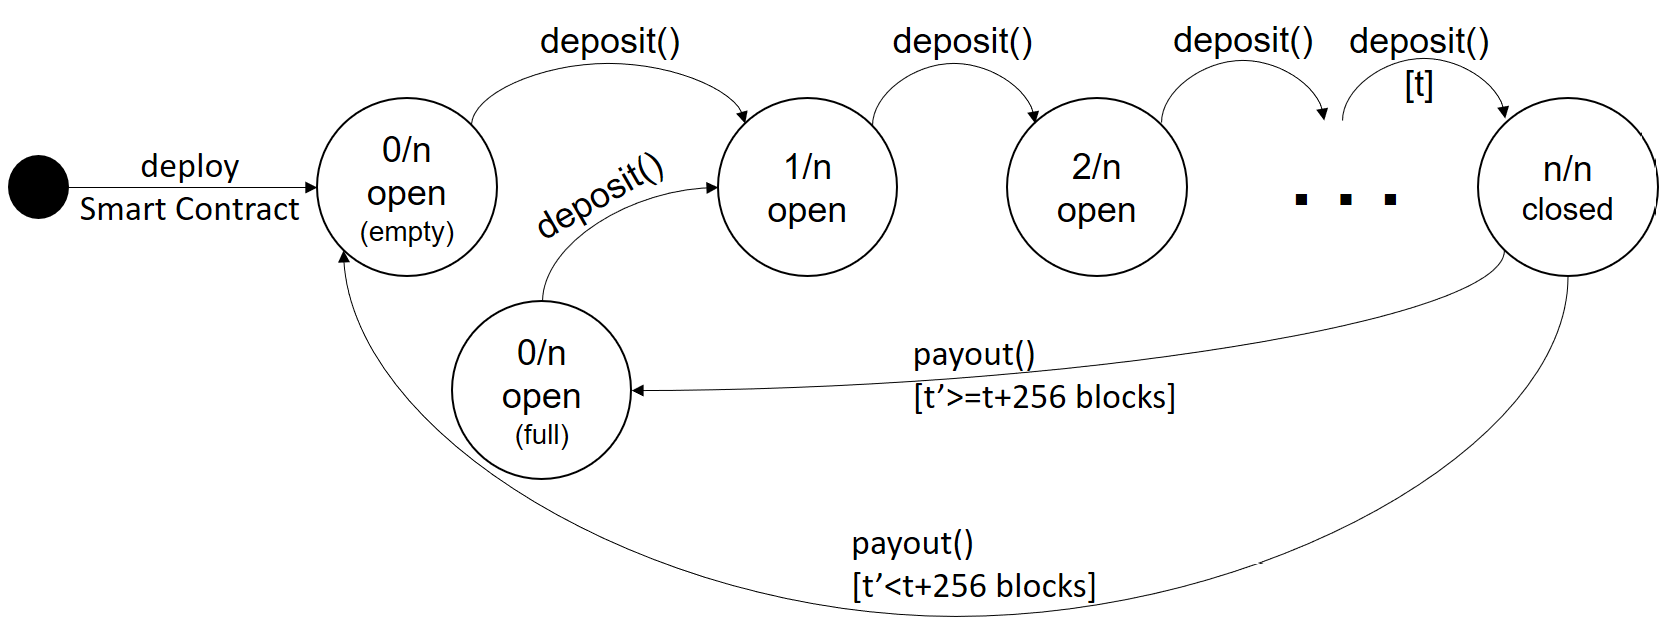
\includegraphics[width=1\linewidth]{Figures/umsetzung_eth/smart_contract_automat}
\decoRule
\caption{Smart Contract Umsetzung}
\label{fig:smart_contract_automat}
\end{figure}

\subsection{Smart Contract Bereitstellung}
Nachdem man den Smart Contract programmiert hat, muss man ihn zu Bytecode kompilieren und anschließen in einer Transaktion an das Ethereum Netzwerk senden. Dazu kann man die von Web3J bereitgestellten Comandline Tool nutzen. Dieses Tool hilft bei der Generierung einer Wallet und erlaubt es aus dem Contract Code eine Java Klasse zu generieren. Dieser Klasse ermöglicht die Interaktion mit dem Smart Contract. 

\begin{lstlisting}[basicstyle=\small]
public void createContract() throws Exception {
  String WALLET_FILENAME = "ethereum.json";
  String WALLET_PASSWORD = "changeit";
  long GAS_LIMIT = 1000000;
  ClassLoader classLoader = getClass().getClassLoader();
  File walletFile = new File(classLoader.getResource(WALLET_FILENAME).getFile());
  Credentials credentials = WalletUtils.loadCredentials(WALLET_PASSWORD, walletFile.getAbsolutePath());
  System.out.println("Account address = " + credentials.getAddress());
  Web3j web3j = Web3j.build(new InfuraHttpService("https://rinkeby.infura.io/" + UserConfiguration.API_KEY));
  BigInteger currentGasPrice = web3j.ethGasPrice().send().getGasPrice();
  TrustlessGambling contract = TrustlessGambling.deploy(web3j, credentials, currentGasPrice, BigInteger.valueOf(GAS_LIMIT)).send();
  String status = contract.getTransactionReceipt().get().getStatus();
  if ("0x1".equals(status)) {
    String address = contract.getContractAddress();
    System.out.println("Contract address = " + address);
    System.out.println("TXN hash = " + contract.getTransactionReceipt().get().getTransactionHash());
    System.out.println("Gas used = " + contract.getTransactionReceipt().get().getGasUsed());
  } else {
    System.out.println("Smart contract could not be deployed.");
  }
}
\end{lstlisting}
Die Ausführung des oben gezeigten Java Codes führt zu der folgenden Ausgabe:

\begin{lstlisting}
Account address = 0x2201f3919589b519135ce977cc0906c9481069b2
Contract address = 0x25c3136145fbd7f3b9217e58e2fabe3eb1928705
TXN hash = 0x06dce3c460b4caa595c5cc0f81ac78e7c70eeb1e89d3e0e6a017ea88e60dbce1
Gas used = 825846
\end{lstlisting}

In einem Blockchain Explorer kann man die Details der vom Full Node erstellten Transaktion\footnote{\url{https://rinkeby.etherscan.io/tx/0x06dce3c460b4caa595c5cc0f81ac78e7c70eeb1e89d3e0e6a017ea88e60dbce1}} und den kompilierten Contract Code\footnote{\url{https://rinkeby.etherscan.io/address/0x25c3136145fbd7f3b9217e58e2fabe3eb1928705\#code}} anschauen.
Alternativ zu Web3J lässt sich der Contract Code mithilfe eines Online Compilers \footnote{\url{https://ethereum.github.io/browser-solidity}} kompilieren und mithilfe des Ethereum Clients namens Mist\footnote{\url{https://github.com/ethereum/mist}} veröffentlichen.

\subsection{Geschäftslogik Webanwendung}

Dieses Kapitel zeigt, wie man in Etherem über einen Full Node mit dem Netzwerk interagieren kann. Die Webanwendung zeigt lediglich lediglich den aktuellen Zustand des Smart Contracts an. Die gesamte Geschäftslogik des Smart Contracts wird vom Etherem Netzwerk ausgeführt. Sollte die Webanwendung aufgrund  technischer Fehler ausfallen, hat dies keinerlei Auswirkung auf das eigentliche Spiel.

TODO 

\iffalse
\begin{enumerate}
\item Es gibt sowohl test als auch mainnet. Unterscheiden sih nur leicht durch protokoll und port. Teil sehen adressen anders aus. Bei ethereum creiert man sich ein wallet und die adresse ist für beide netzwerke gültig.
\item Auf dem testents gibts faucts für entwickler, die einem ein wenig testnet cryptowährung überweisen nachdem man ein captcha gelöst hat. Problem öffters mal down.
\item Bei ethereum hatte ich das typische Java problem, dass die web3jlib eine neuere verion vewendete als der Jboss Wildfly. Daher musste ich den jboss hochziehen
\item Neuer wildfly benutzt port /127.0.0.1:9990 den auch ein nvidea network service verwendet. den musste ich dann erst abschiessen.
\end{enumerate}
\fi

\subsection{Grafische Benutzeroberfläche}

Das folgende Beispiel betrachtet einen frisch auf dem Ethereum Rinkeby Testnetzwerk bereitgestellten Smart Contract.


\begin{figure}[H]
\centering
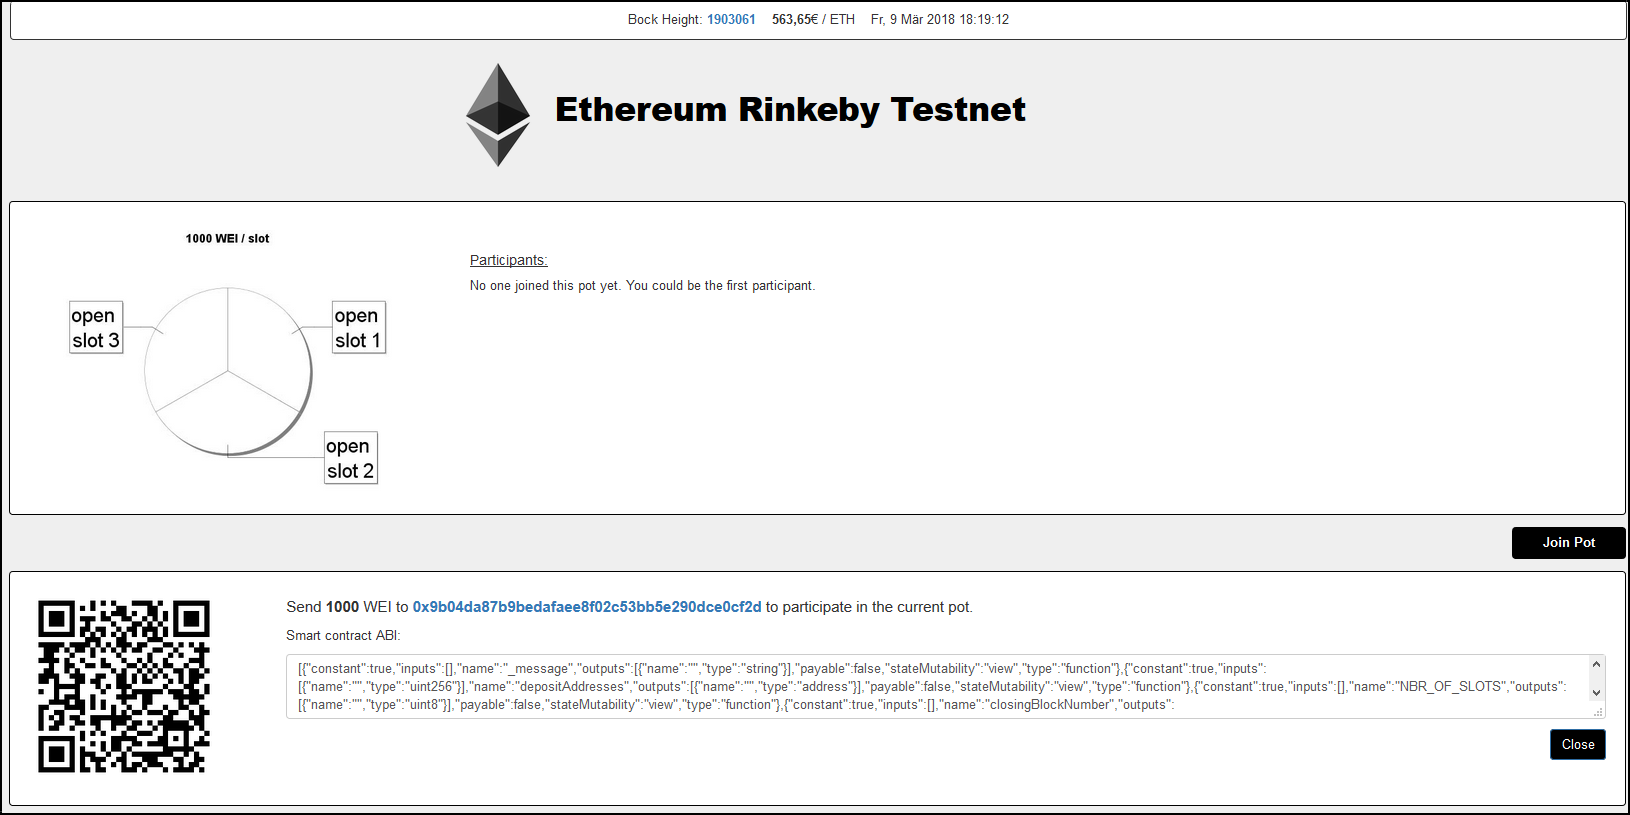
\includegraphics[width=1\linewidth]{Figures/eth_gui/ETH_pot_empty}
\decoRule
\caption{Leerer Topf}
\label{fig:ETH_pot_empty}
\end{figure}
Abbildung \ref{fig:ETH_pot_empty} zeigt einen Topf mit 3 freien Plätzen. Um dem Spiel beizutreten, muss der Spieler den Betrag von 1000 WEI (kleinste Ether Einheit) an den Smart Contract senden. Genau wie bei Bitcoin wird dem Nutzer ein QR-Code angezeigt, der die Übermittlung der Daten in einen Smartphone Client erleichtert. Das \textbf{E}thereum \textbf{I}mprovement \textbf{P}roposal Nummer 681\citep{eip21} legt die Kodierung der Daten fest.
Folgende Daten sind in dem QR Code enthalten:\\ ''ethereum:0x9b04da87b9bedafaee8f02c53bb5e290dce0cf2d/deposit?value=1000''. In diesem Beispiel verwenden wir für die Interaktion mit dem Netzwerk keinen Smartphone Client sondern die Webanwendung namens ''My Ether Wallet''\footnote{\url{https://www.myetherwallet.com/\#contracts}}. Diese benötigt für die Interaktion mit dem Smart Contract sowohl die Contract Adresse als auch das \textbf{A}pplication \textbf{B}inary \textbf{I}nterface.


\begin{figure}[H]
\centering
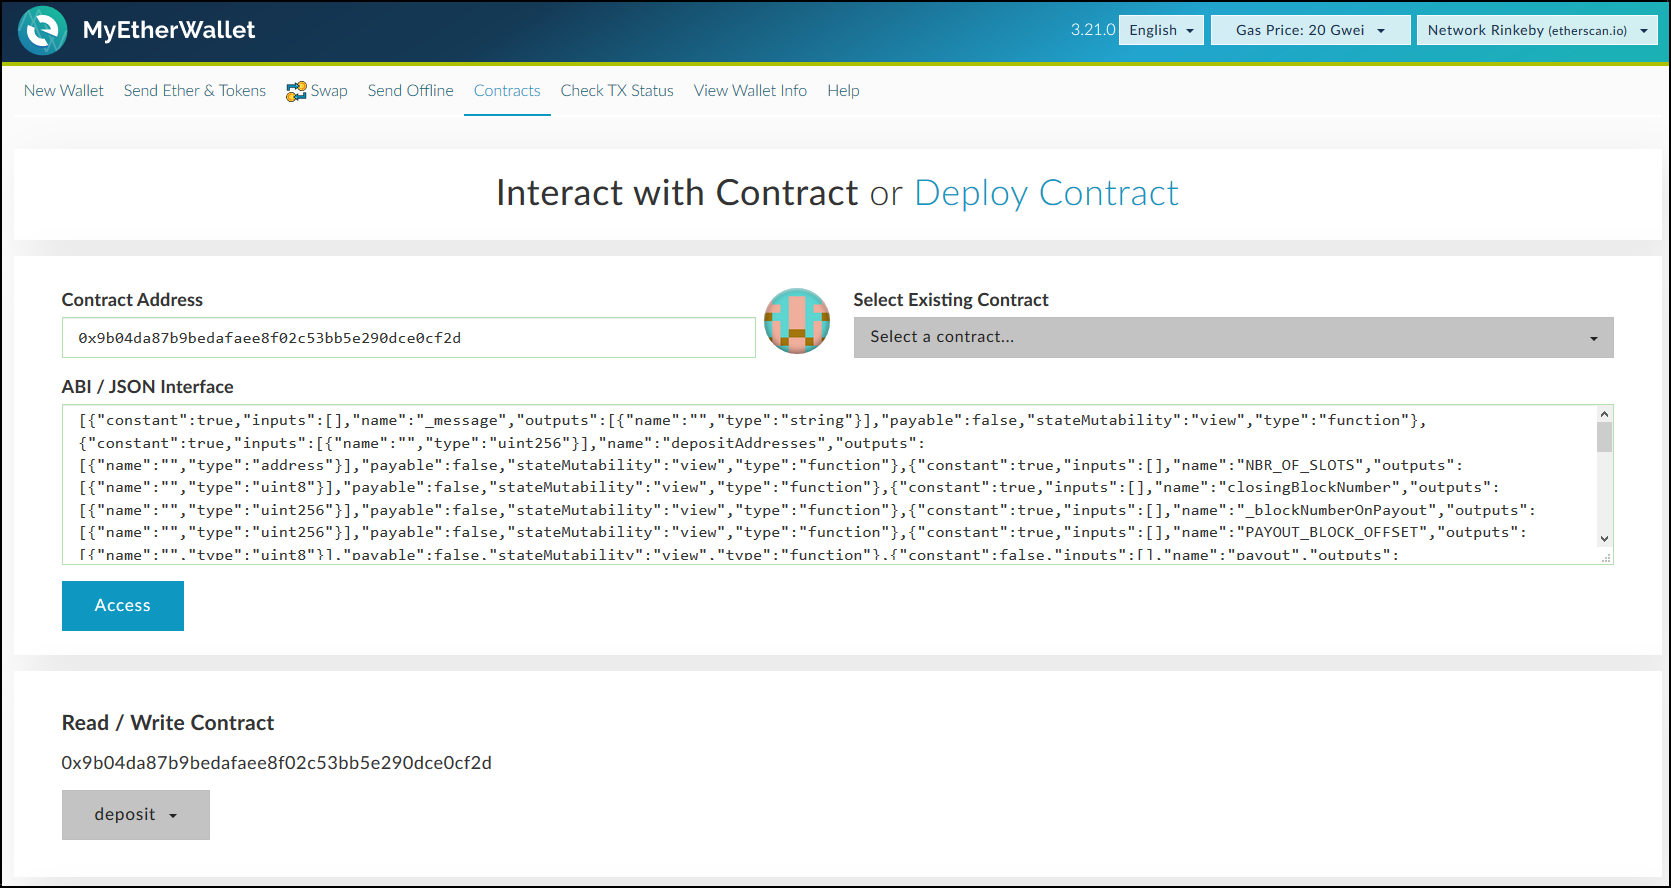
\includegraphics[width=1\linewidth]{Figures/eth_gui/ETH_wallet}
\decoRule
\caption{My Ether Wallet}
\label{fig:ETH_wallet}
\end{figure}

Nachdem der Nutzer diese wie in Abbildung \ref{fig:ETH_wallet} eingegeben hat kann er über eine Dropdown-Liste die gewünschte Funktion des Smart Contracts aufrufen.

\begin{figure}[H]
\centering
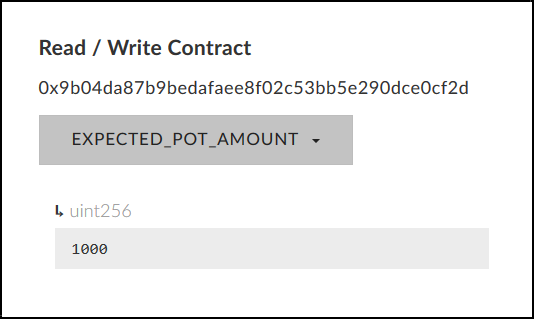
\includegraphics[scale=0.85]{Figures/eth_gui/ETH_wallet_expected_amount}
\decoRule
\caption{Aufruf der \code{EXPECTED POT AMOUNT} Funktion}
\label{fig:ETH_wallet_expected_amount}
\end{figure}

Abbildung \ref{fig:ETH_wallet_expected_amount} zeigt den Aufruf der Funktion auf, die zurückgibt, welchen Geldbetrag der Smart Contract vom Spieler erwartet. Da es sich lediglich um einen lesenden Zugriff handelt, wird keine Transaktion ans Netzwerk gesendet, beziehungsweise in die Blockchain geschrieben. Es fallen somit keine Transaktionskosten an.

\begin{figure}[H]
\centering
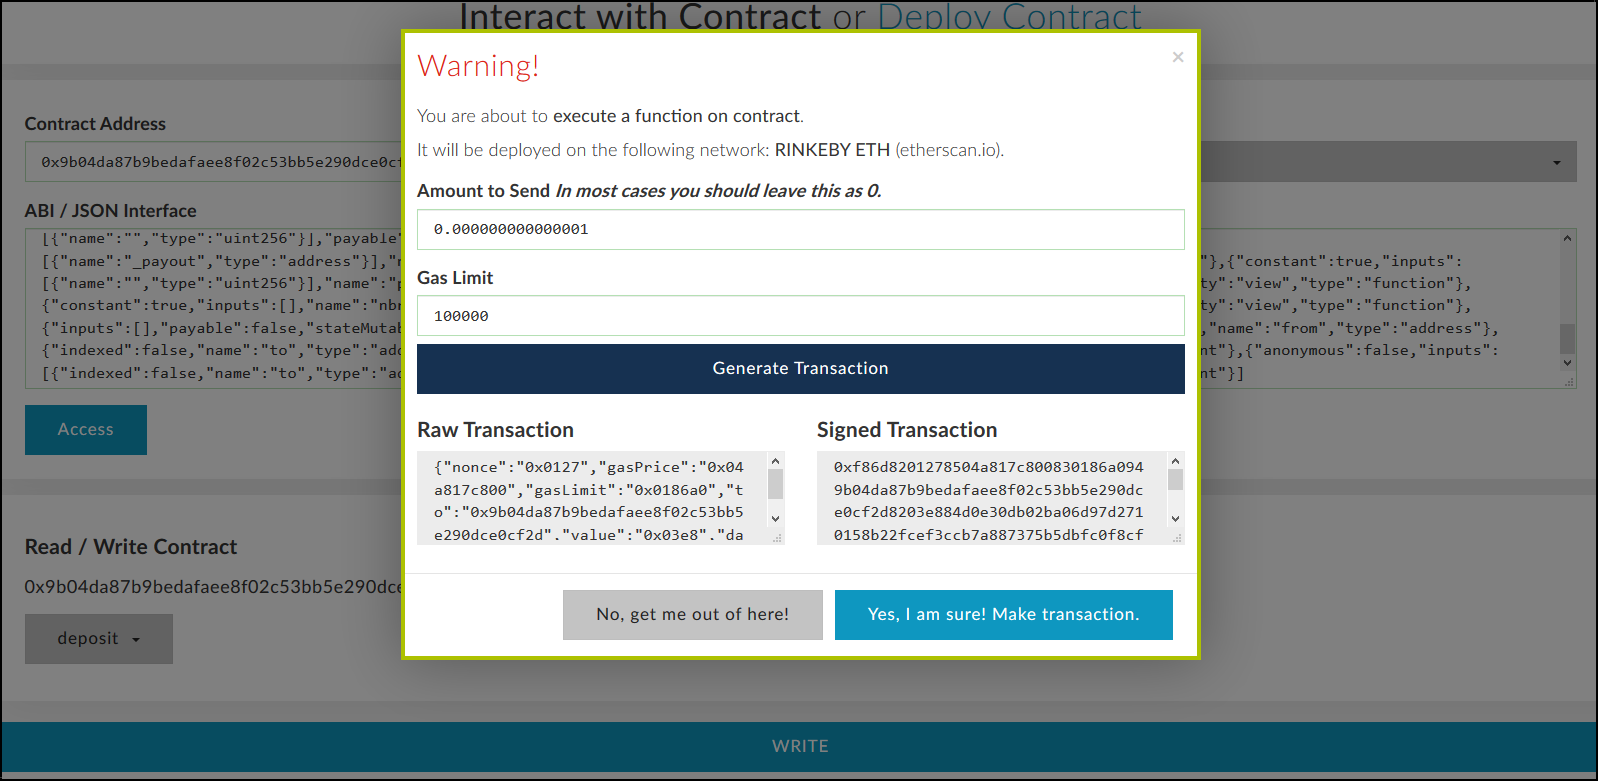
\includegraphics[width=1\linewidth]{Figures/eth_gui/ETH_wallet_deposit}
\decoRule
\caption{Aufruf der \code{deposit} Funktion}
\label{fig:ETH_wallet_deposit}
\end{figure}

Da der Nutzer nun nachgeprüft hat, dass der Smart Contract wirklich Zahlungen von 1000 WEI erwartet, kann er die \code{depsoit} Funktion mit diesem Betrag aufrufen.
Die Wallet Webseite erwartet den Betrag in der Einheit Ether. Die geforderten 1000 WEI entsprechen 0.000000000000001 Ether. Die Umrechnung kann der Spieler mittels eines Online Konverters\footnote{\url{https://etherconverter.online/}} durchführen.
Nun muss die erstellte Transaktion nur noch signiert werden. Der Nutzer kann der Webseite dazu seinen privaten Schlüssel mitteilen oder die Signierung eigenständig durch ein sogenanntes Hardware Wallet durchführen. Die Herausgabe seines privaten Schlüssels an eine Webseite ist aus sicherheitstechnischer Sicht keine gute Praktik. Sollte der Webseitenbetreiber böse Absichten haben oder die Webseite gehackt werden, führt dies zum Verlust des durch den Schlüssel kontrollierten Geldes. Eine sichere Variante ist die Verwendung eines Hardware Wallets. Dieses speichert alle privaten Schlüssel und führt die Signatur eigenständig durch. Der verwendete private Schlüssel verlässt somit niemals das Gerät. 

\begin{figure}[H]
\centering
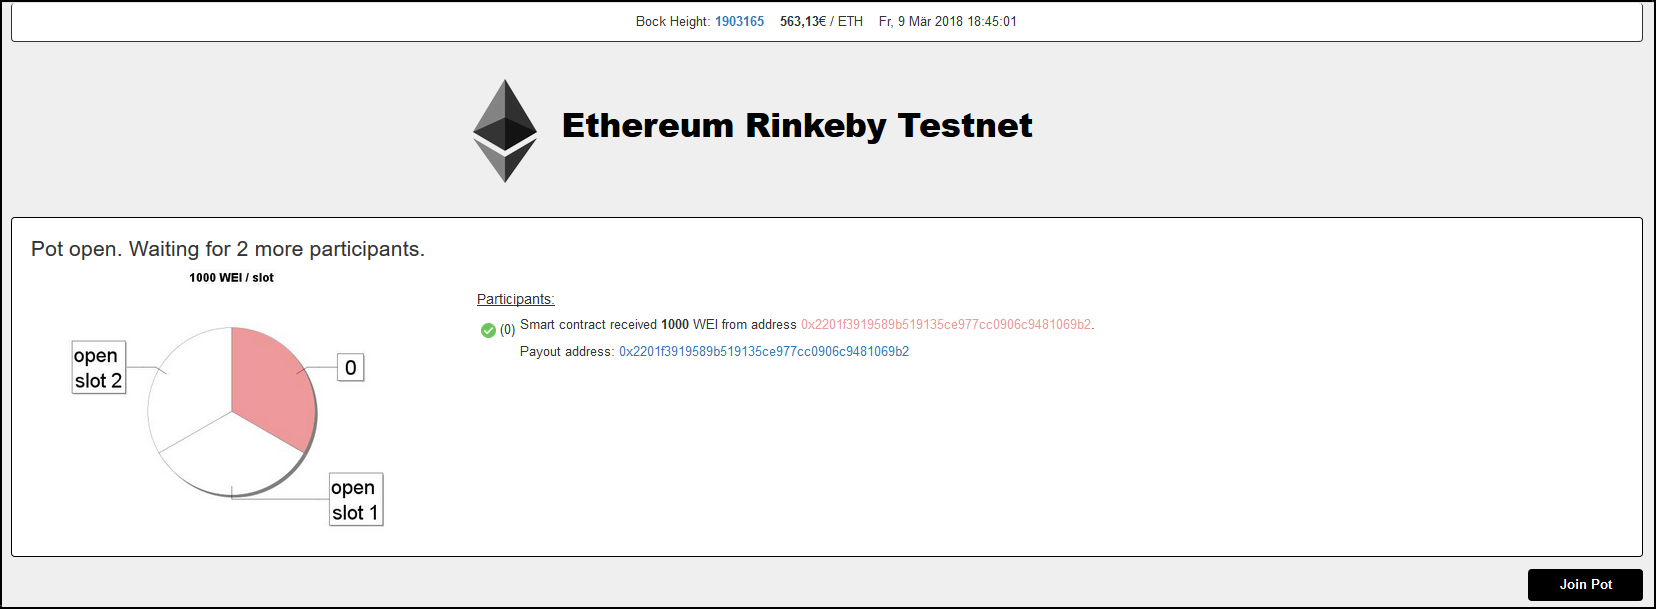
\includegraphics[width=1\linewidth]{Figures/eth_gui/ETH_pot_1}
\decoRule
\caption{Eingang der ersten Zahlung}
\label{fig:ETH_pot_1}
\end{figure}

Abbildung \ref{fig:ETH_pot_1} visualisiert den Zustand des Smart Contracts nachdem die erste Einzahlungstransaktion in die Blockchain aufgenommen wurde.

\begin{figure}[H]
\centering
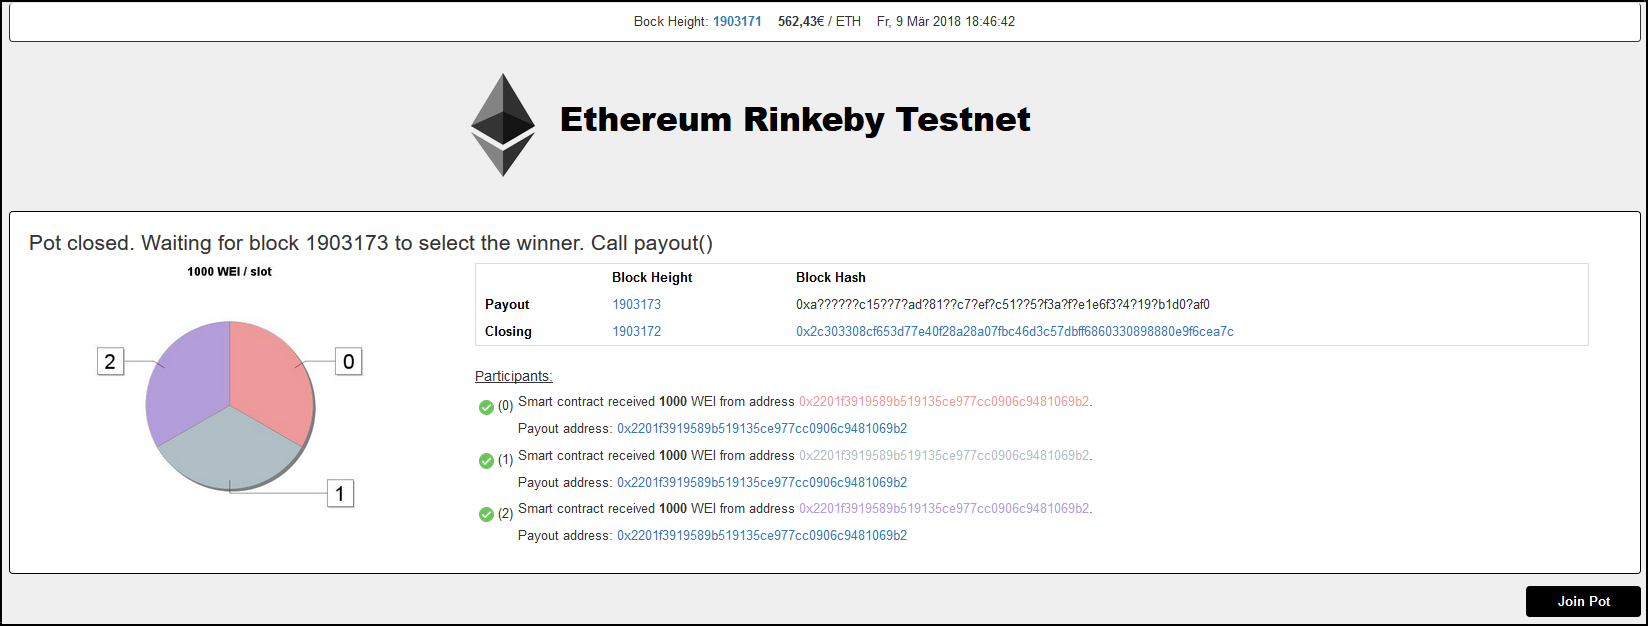
\includegraphics[width=1\linewidth]{Figures/eth_gui/ETH_pot_closed}
\decoRule
\caption{Topf geschlossen}
\label{fig:ETH_pot_closed}
\end{figure}

Abbildung \ref{fig:ETH_pot_closed} visualisiert den Zustand des Smart Contracts nachdem die letzte Einzahlungstransaktion in die Blockchain aufgenommen wurde. Der Smart Contract hat den Topf geschlossen und wartet nun, dass einer der Spieler die \code{payout} Funktion aufruft.

\begin{figure}[H]
\centering
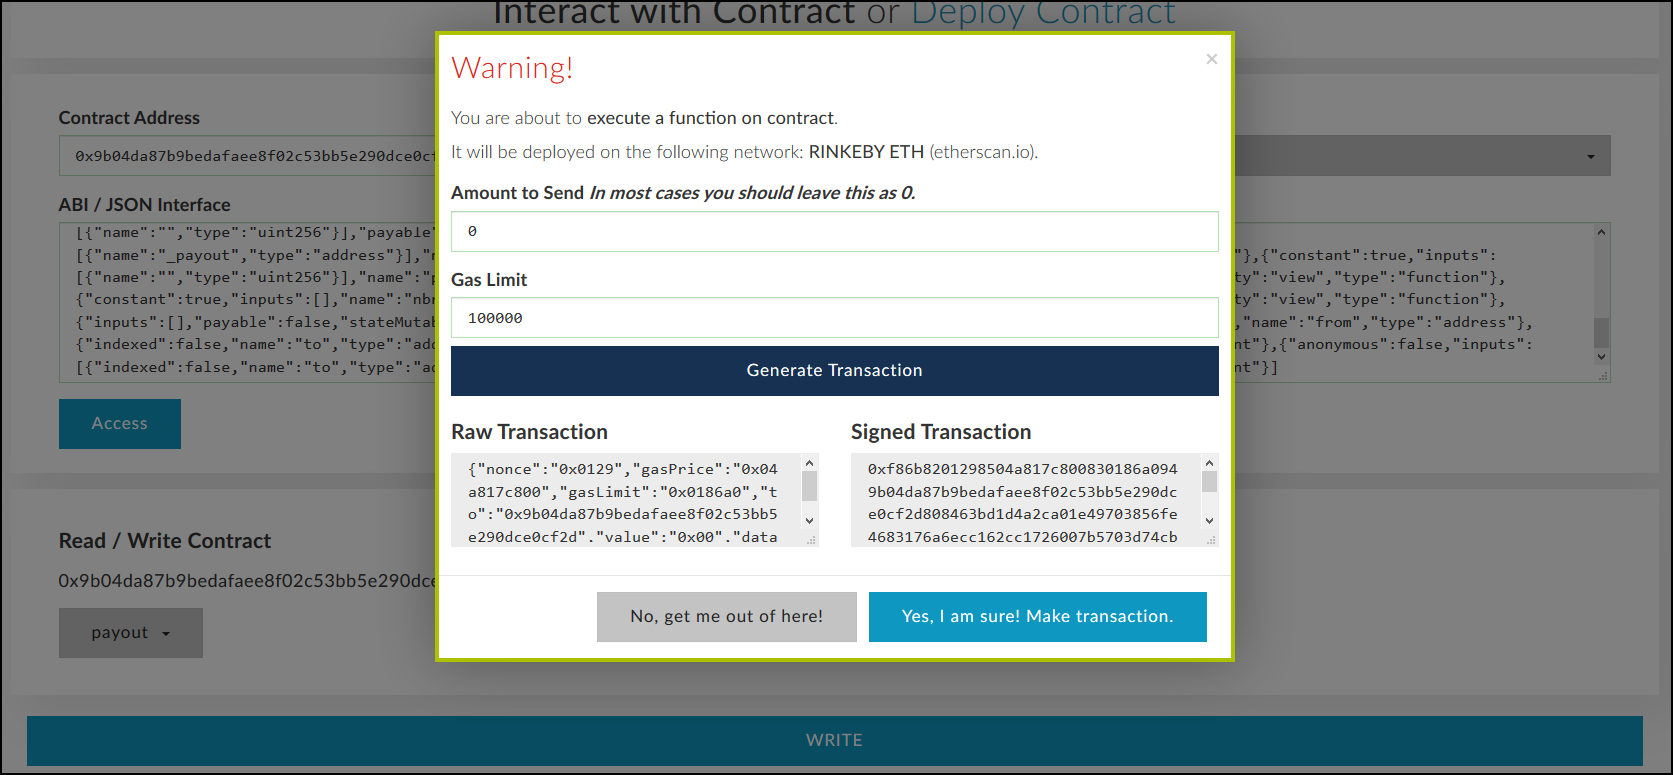
\includegraphics[width=1\linewidth]{Figures/eth_gui/ETH_wallet_payout}
\decoRule
\caption{Aufruf der \code{payout} Funktion}
\label{fig:ETH_wallet_payout}
\end{figure}

In Abbildung \ref{fig:ETH_wallet_payout} ist gezeigt wie ein Spieler die  \code{payout} Funktion aufruft. Durch den Aufruf dieser Funktion wird der Gewinner ausgewählt, die Auszahlung getätigt und der Topf wieder geöffnet.

\begin{figure}[H]
\centering
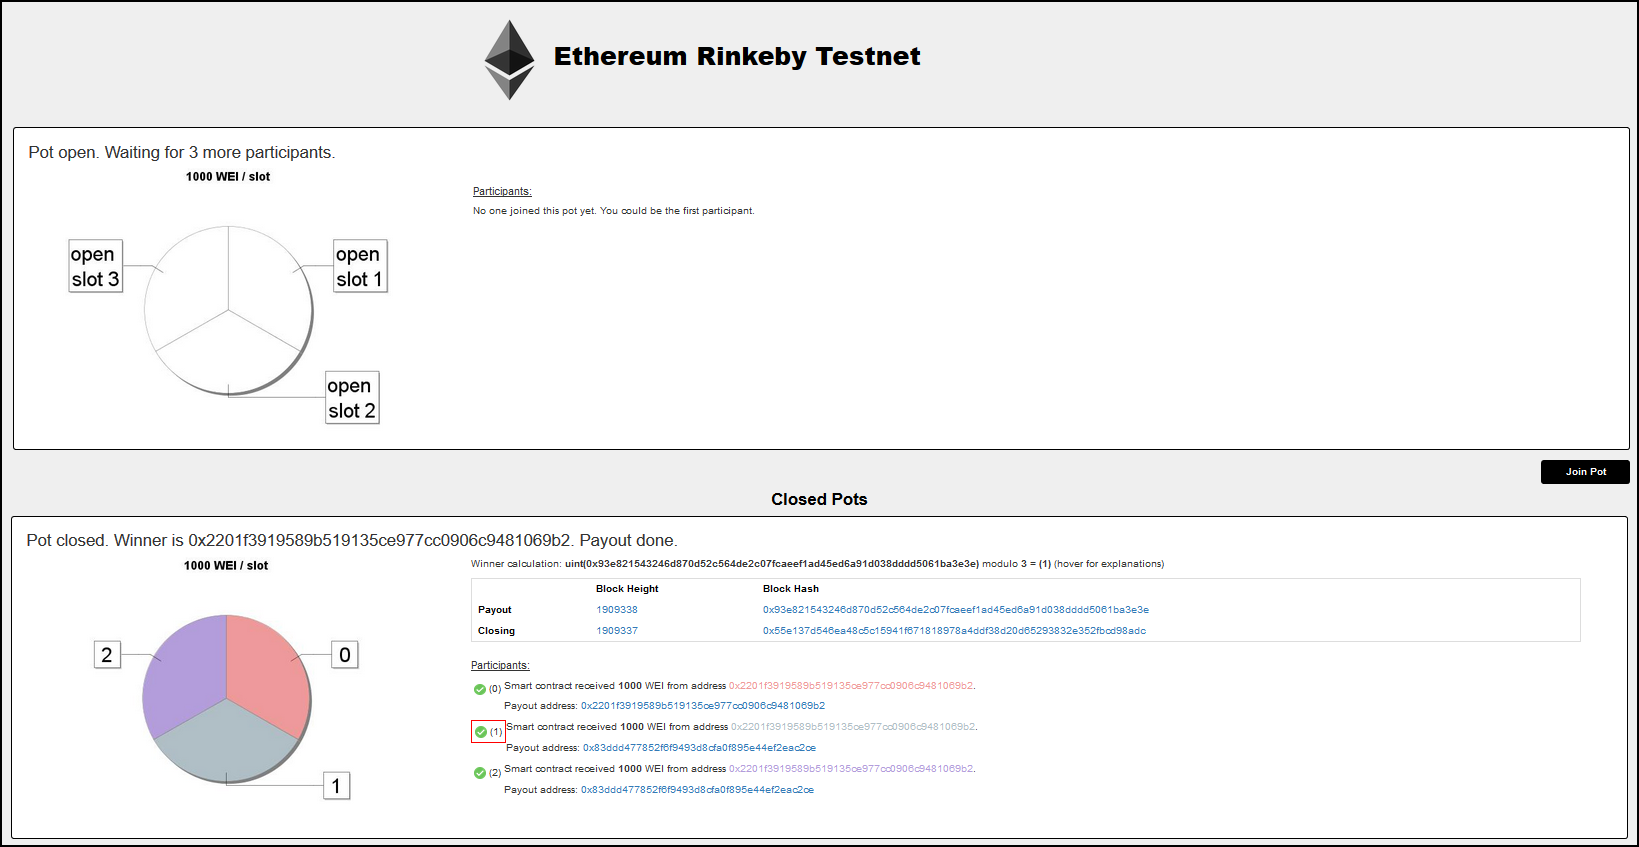
\includegraphics[width=1\linewidth]{Figures/eth_gui/ETH_pot_finished}
\decoRule
\caption{Gewinner ausgewählt}
\label{fig:ETH_pot_finished}
\end{figure}

Abbildung \ref{fig:ETH_pot_finished} zeigt den Gewinner des alten Topfs und den neu geöffneten Topf.